\section{Are emerging-market owners constrained?}\label{sec:constraints}

Equal survival at equal quality does not rule out owner constraints: constrained owners might keep their patents as
long as others but get less from them, or drop patents that would be worth keeping in other hands. Four tests look
for constraints directly. Figure~\ref{fig:constraints} summarises them.

\begin{figure}[!htbp]
\centering
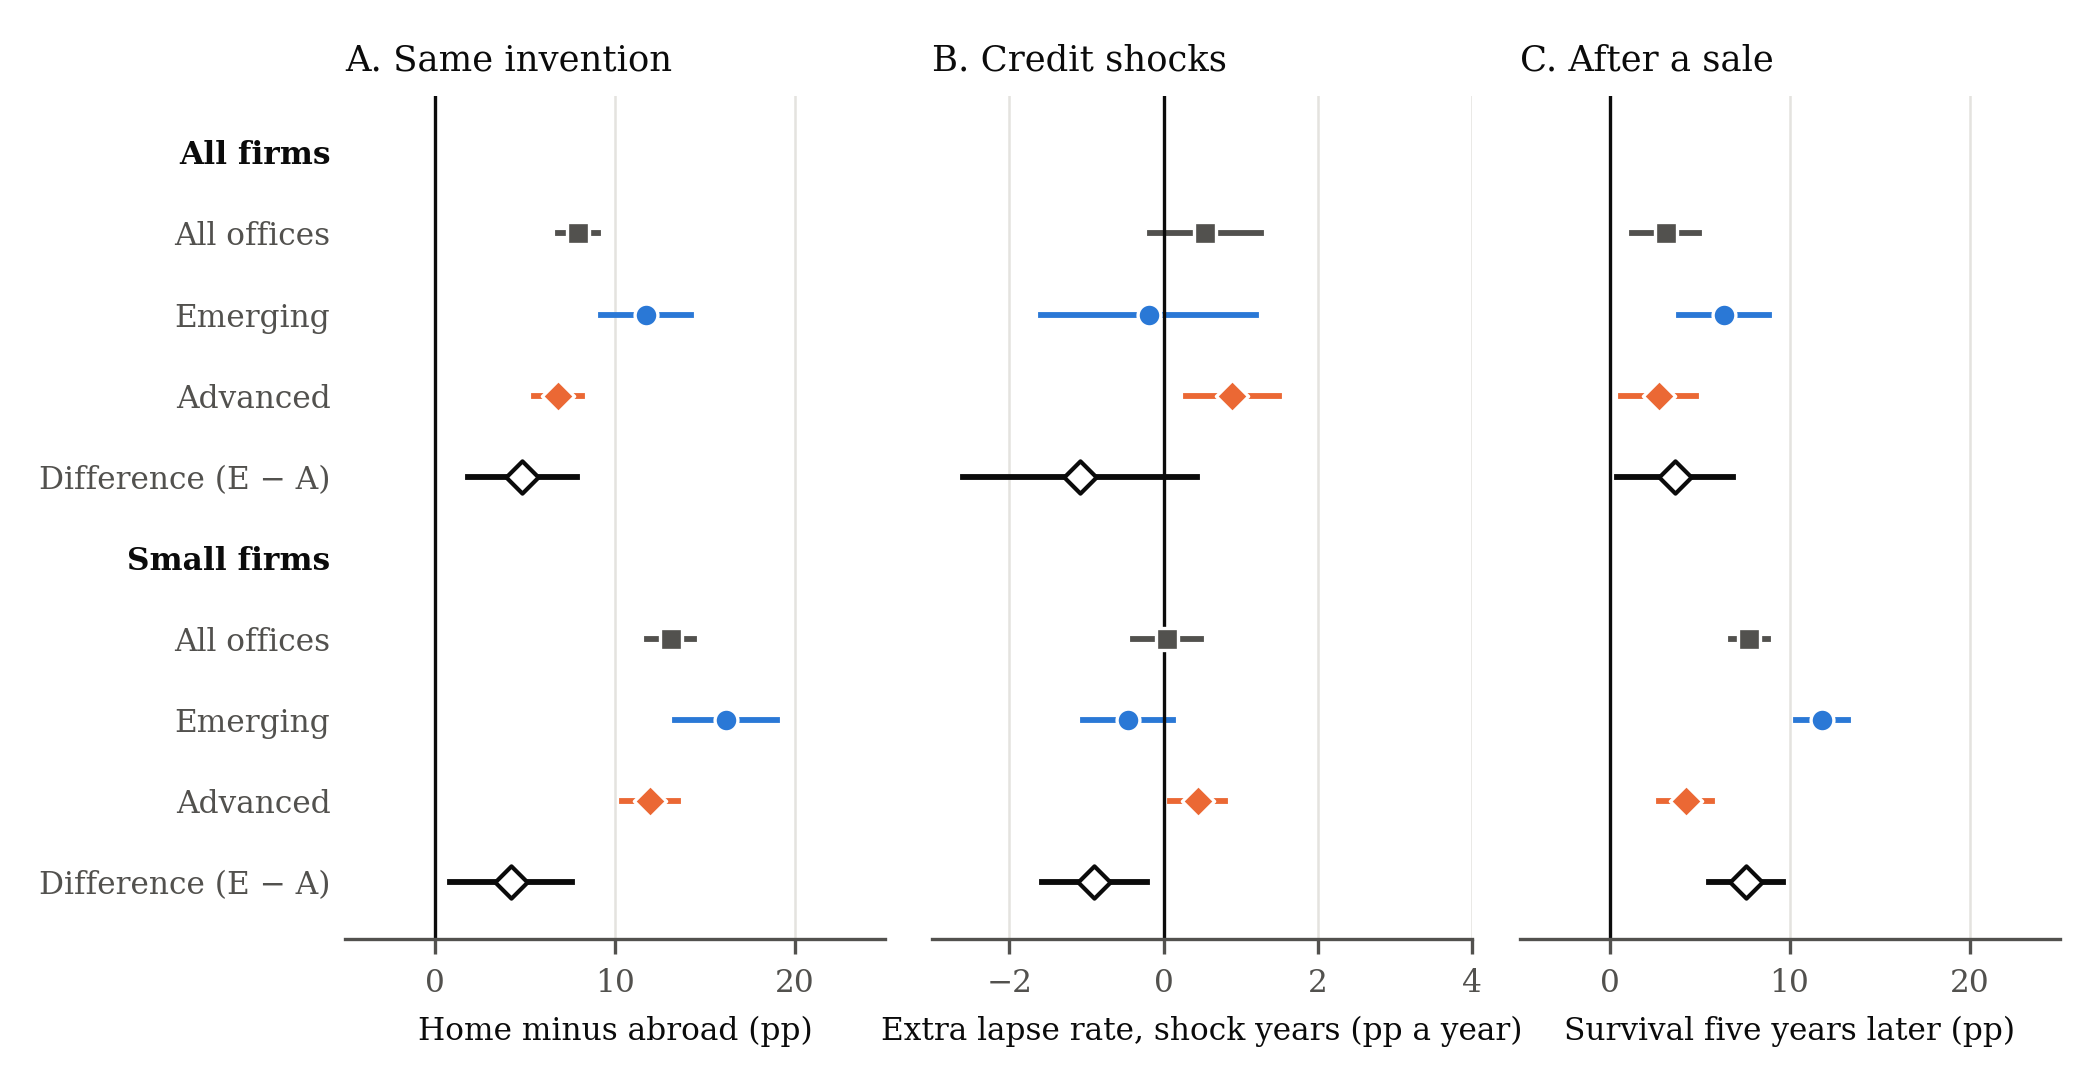
\includegraphics[width=0.95\textwidth]{figures/fig5_constraints.png}
\caption{Four tests for owner constraints}\label{fig:constraints}
\figurenotes{Point estimates with 95\% confidence intervals; circles: emerging-market offices or owners, diamonds:
advanced-economy ones. A: inventions with granted patents at home and in another study office; survival eight years
after grant of the home patent minus the foreign ones, small firms (1--9 inventions) minus larger firms from the same
country, with patent-family and office $\times$ year fixed effects; the Czech Republic has too few small-firm
inventions patented abroad. B: interaction of credit-shock year, small owner and domestic owner in yearly lapse rates,
with office $\times$ year, office $\times$ age $\times$ citation-tercile and office $\times$ owner $\times$ domestic
effects. C: survival five years after a sale at ages 4--8 (landmark design, citations counted up to the landmark age);
all sellers, and the extra for small domestic sellers in each group of offices; Taiwan and the Czech Republic record no
transfers. D: elasticity of the yearly lapse probability with respect to the fee, small firms against firms with 100
or more inventions (China: intent to treat, 85\% discount window; US: stage-specific maintenance-fee changes); the
Korean and French discounts are not identified (Appendix Table~\ref{tab:fees}). Standard errors clustered by owner
(A, C, D) or office $\times$ year (B).}
\end{figure}

\paragraph{Same invention, home and abroad.} Inventions patented both at home and in another study office hold the
technology fixed. With patent-family fixed effects, I compare how much longer small firms keep the home patent than
the same invention's foreign patents, relative to larger firms from the same country. If small emerging-market firms
found their home patents hard to use, they would drop them first. They do the opposite (panel A): small firms keep
the home patent relatively longer in China, by 10.6 (3.7) points, and Korea, by 10.7 (1.8), as in Japan (15.7),
France (7.2) and the United States (2.8); in Taiwan the difference is close to zero and in Russia it is imprecise
(Appendix Table~\ref{tab:same}). Small owners everywhere economise on the expensive foreign patent first.

\paragraph{Credit shocks.} If finance were binding, credit crunches should raise small domestic firms' lapses. In a
patent-year panel with country-specific shock years (banking crises and documented credit crunches;
\citealp{LaevenValencia2018}), the interaction of shock, small owner and domestic owner is 0.32 points a year (0.86)
in the emerging-market offices and 0.16 (0.51) in the advanced-economy ones (panel B; Appendix
Table~\ref{tab:credit}). Office $\times$ year effects absorb fee changes and recording practices.

\paragraph{Fees.} Fee changes test cash constraints at renewal time directly. China's 85\% fee reduction for small
owners, whose window was extended from three to six fee-years in 2016 and to ten in 2018, lowers small firms' lapse
rate only slightly: an implied elasticity of 0.05 (intent to treat, since take-up is not observed). Small US firms
respond to stage-specific maintenance-fee changes with an elasticity of about 0.26 (panel D). Small emerging-market
firms are not more fee-sensitive than small US firms.

\paragraph{Sales.} One result points to owner capacity at the margin. In a landmark design (patents alive and not
yet sold at ages 4--8, sold in the next year or not, outcome alive five years later, with citations counted only up
to the landmark age), a sale raises survival by 4.9 (0.7) points on average, by a further 6.9 (1.0) for small
emerging-market firms and not at all for small advanced-economy firms, 0.0 (1.0) (panel C; Appendix
Table~\ref{tab:credit}, panel B). Buyers select good patents everywhere, so the level of the premium is not causal; the
extra premium for small emerging-market sellers is the informative part. In China it is largest for sales to other
firms; in Russia there is none. Taiwan and the Czech Republic record no ownership transfers.
